\documentclass[11pt]{article}
\usepackage{tikz}
%\usepackage{xfrac}
%\usepackage{hyperref}
%\usepackage[export]{adjustbox}
\def\checkmark{\tikz\fill[scale=0.4](0,.35) -- (.25,0) -- (1,.7) -- (.25,.15) -- cycle;} 
\usepackage{proj} 	% pull in style header
\usepackage{array}
\usepackage{sectsty}
\usepackage{soul}
\usepackage{float}
\usepackage{multirow} 
\usepackage{gensymb}
\restylefloat{table}

\lhead{ECE544: Embedded Systems on FPGAs}


%----------------------------------------------------------------------------------------
%	TITLE SECTION
%----------------------------------------------------------------------------------------


\newcommand{\horrule}[1]{\rule{\linewidth}{#1}} % Create horizontal rule command with 1 argument of height

\title{	
\normalfont \normalsize 
\textsc{\LARGE Portland State University}\\[1.5cm] % Name of your university/college
\textsc{\Large Embedded Systems on FPGAs}\\[0.5cm] % Major heading such as course name
\textsc{\large ECE544}\\[0.5cm] % Minor heading such as course title
%\textsc{Portland State University} \\ [25pt] % Your university, school and/or department name(s)
\horrule{1.2pt} \\[0.4cm] % Thin top horizontal rule
\huge Autonomous Robot Car \\ % The assignment title
\horrule{1.2pt} \\[0.5cm] % Thick bottom horizontal rule
}

%----------------------------------------------------------------------------------------
%	AUTHOR SECTION
%----------------------------------------------------------------------------------------


\begin{document}
\author{Erik Rhodes \and Caren Zgheib} % Your name
\maketitle % Print the title
\thispagestyle{empty}
\cfoot{\textit{Page \thepage { of} \pageref{LastPage}}}
\lhead{ECE544}
\chead{Final Project}
\rhead{Erik Rhodes \& Caren Zgheib}


\begin{figure}[h]\centering
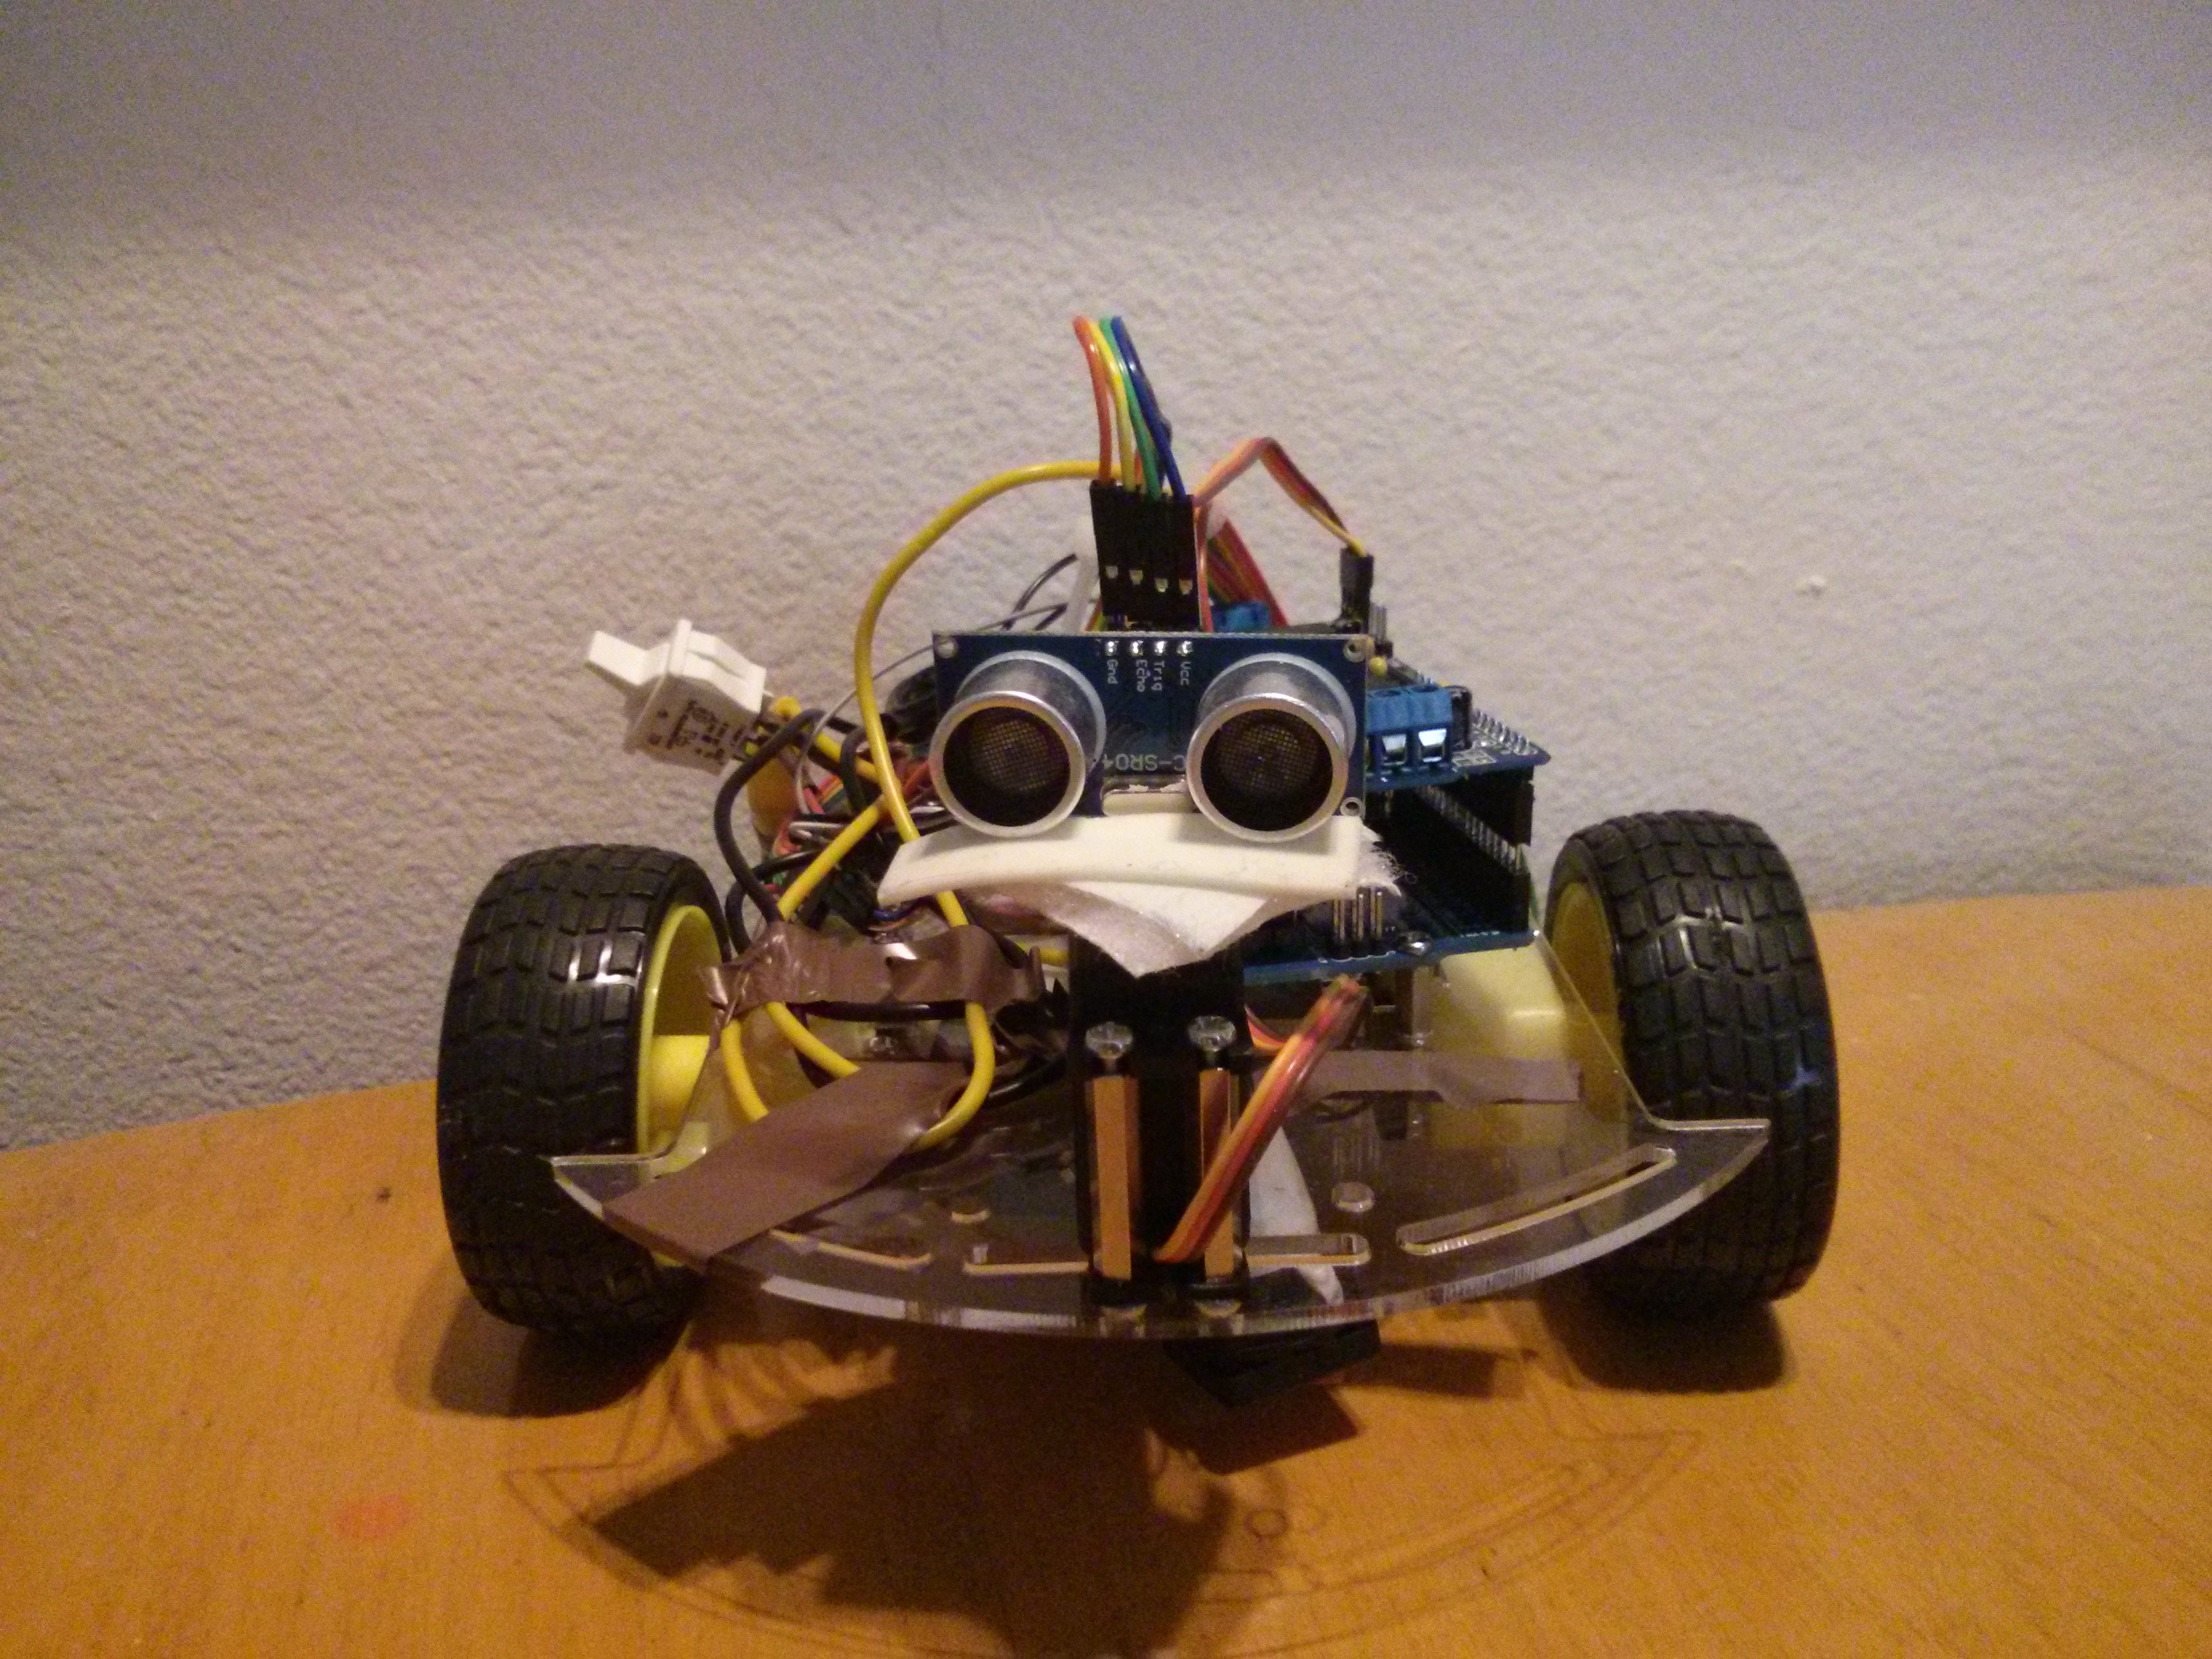
\includegraphics[height=0.65\textwidth]{images/bot_front.jpg}
		\label{bot_front}
	\end{figure}
	
\tableofcontents
\newpage

\section{Introduction} 
We created an autonomous robot car (SaMMY) that can successfully navigate its way through a given area without hitting any objects . It uses the popular \textbf{Arduino} platform and libraries along with a ultrasonic sensor for object detection. 

%TODO 
% Me: Block diagram of arduino (mockup)
% Caren or me: Other flowcharts, diagrams?

\section{Hardware Components}
There are many different components needed to successfully and robustly create an autonomous robot.  The bulk of our design used a robot kit we ordered online (ref).  We also added various parts to make the production time more convenient, including switches, additional batteries, and various cables.  The important components can be seen in Figure \ref{diagram} and are described in Table \ref{components}.


	\begin{figure}[h]\centering
	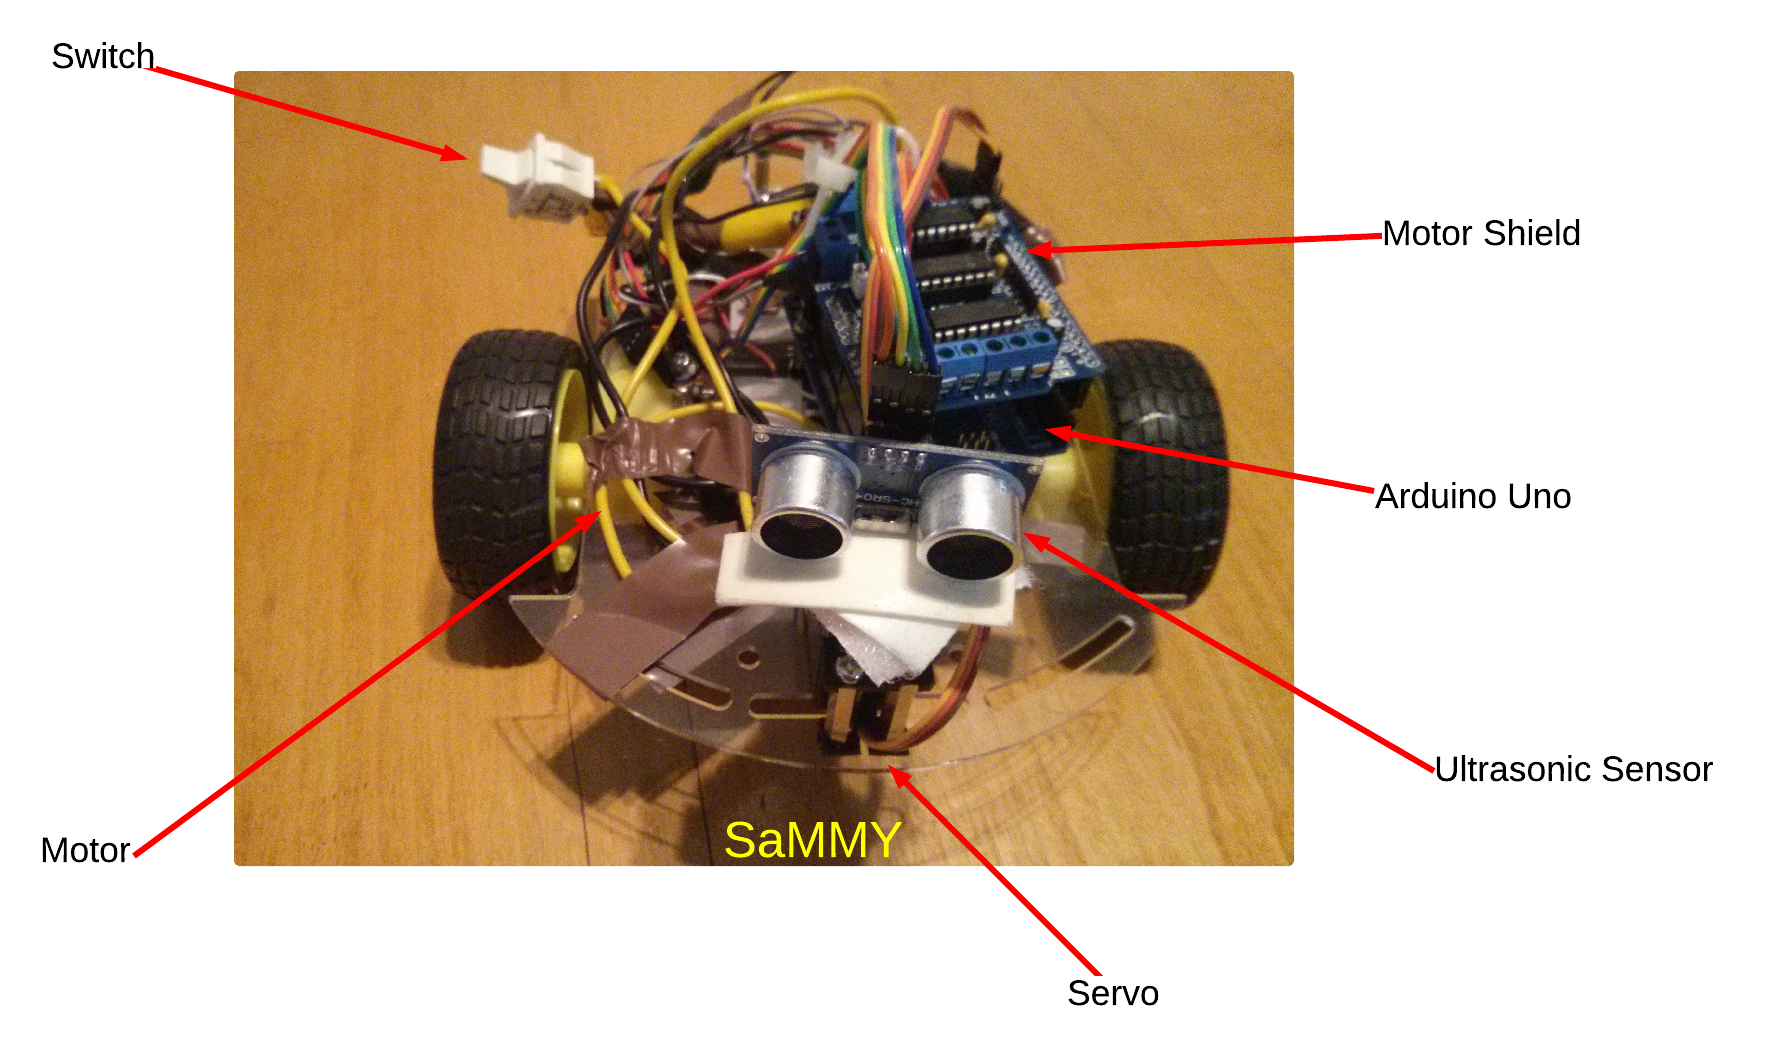
\includegraphics[height=0.57\textwidth]{images/bot_diagram.png}
	\caption{Block Diagram of Control System}
		\label{diagram}
	\end{figure}

	\begin {table}[h]
	\begin {center} 
	%\vspace{15pt}
	
	\begin{tabular}{||l|c|c||}\hline
	%\multicolumn{3}{ |c| }{\textbf{Component List}} \\\hline	
		\textbf{Part Name}	&	\textbf{Function}	&	\textbf{Details}		\\\hline
		1. Motor 		&	Drives wheels				&	N/A 		\\\hline
		2. RadioShack\textsuperscript{\textregistered} Standard Servo		&	180\degree rotation 		&	\url{http://shack.net/Ty2VB4} 		\\\hline
		3. Ultrasonic Ranging Module HC-SR04		&	Object detection	&	\url{http://bit.ly/1lhqwjI}	 	\\\hline
		4. Arduino Uno		&	Microcontroller Board			&	\url{http://bit.ly/1gBB1NG} 		\\\hline
		5.	L293D Motor Driver Shield	&	Controls motors &	\url{http://bit.ly/1uILISF}	\\\hline
		6. Switch	&	On/Off power button &	N/A	\\\hline
		7. Batteries (not pictured) & 	9V AA External Power & 	For Arduino/motors/servo \\\hline

		
	\end{tabular}
		\caption {Hardware Components List} \label{components}
	\end{center}
	\end{table} 		
	
Assembling the kit took a fair amount of time.  We added a switch, soldered pins onto the motor shield for the sonar sensor, added the motor shield, changed the weight a few different times, and taped the battery holder to ensure the batteries wouldn't get displaced. Figure \ref{block} shows how each part was connected to the motor shield, which sits on top of the Arduino.

	\begin{figure}[h]\centering
	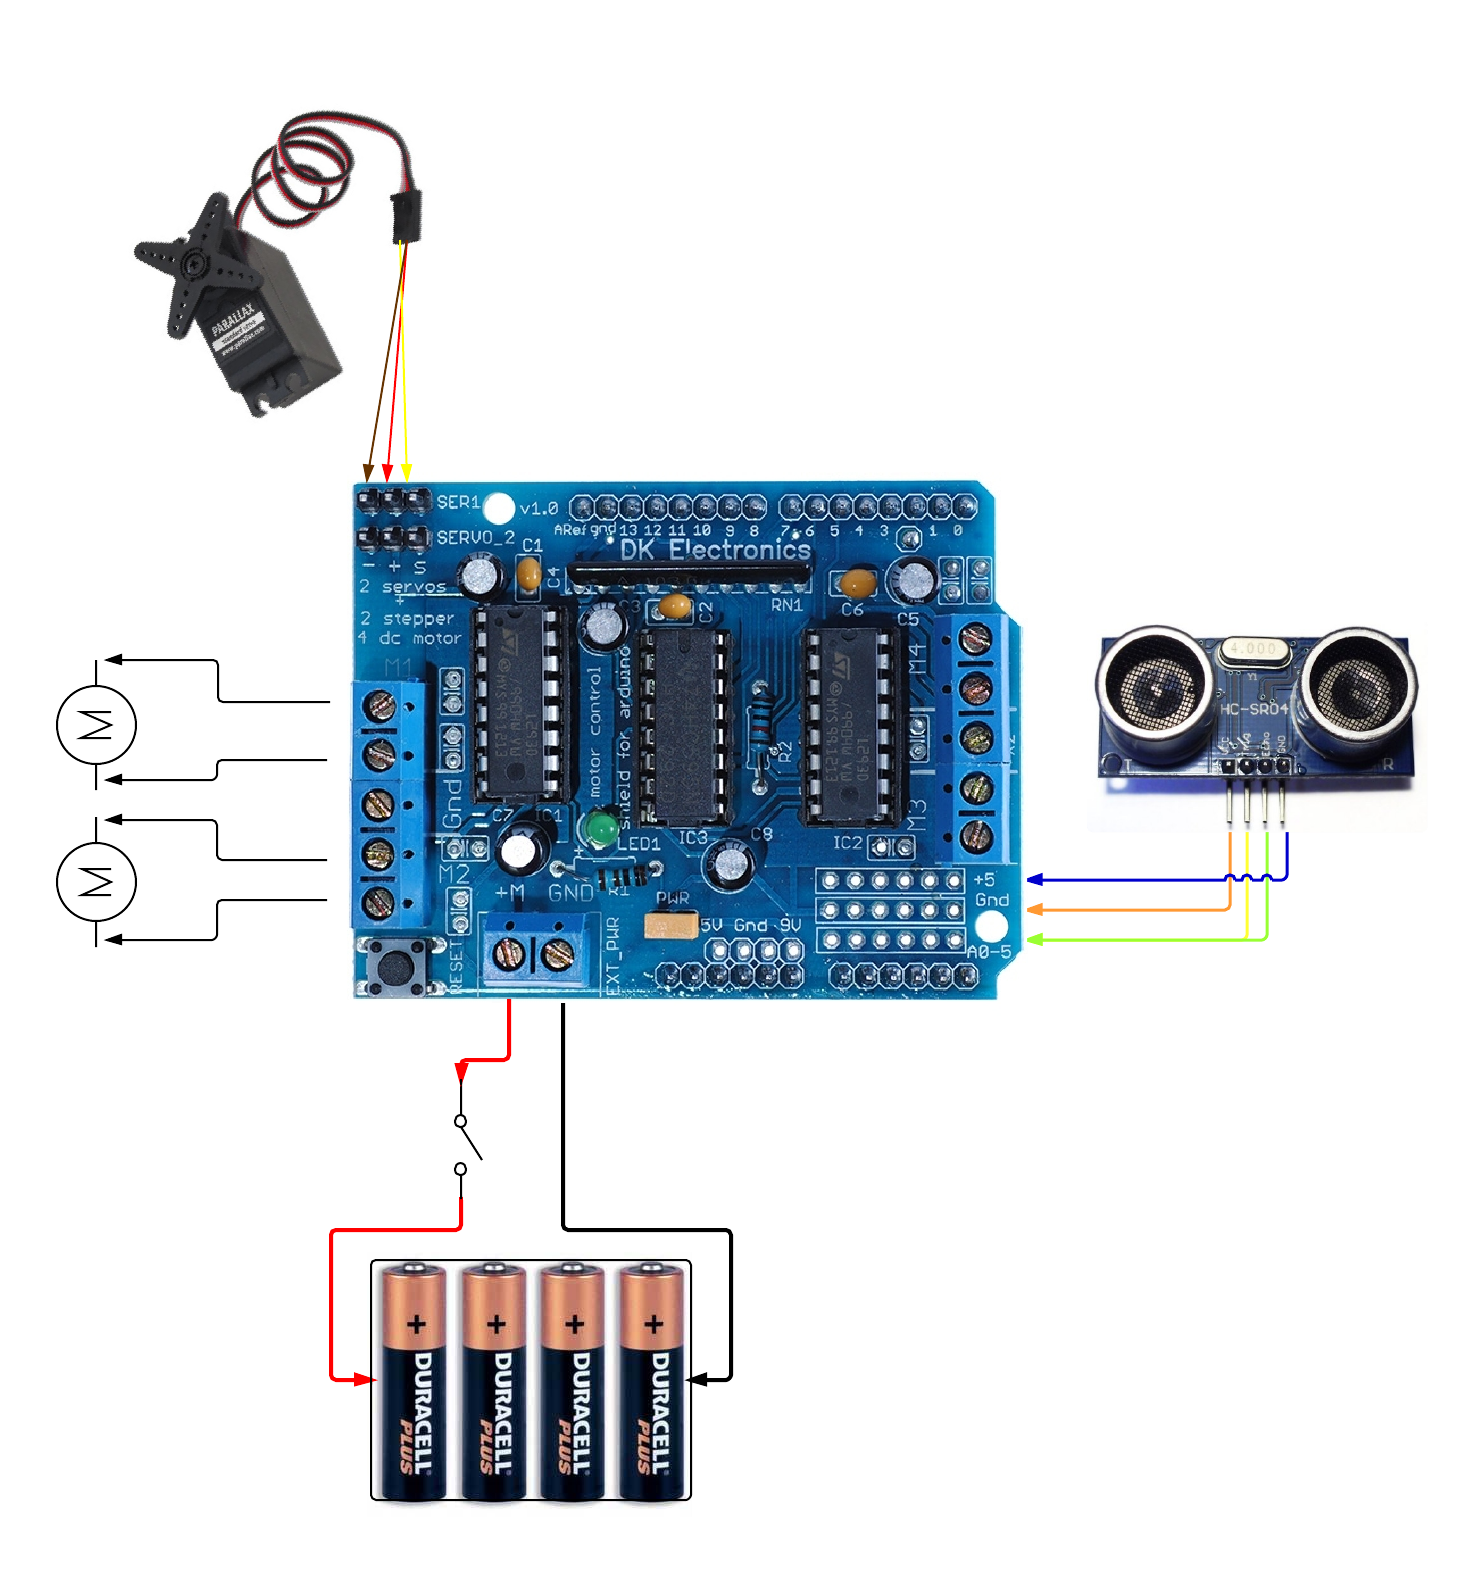
\includegraphics[height=0.85\textwidth]{images/block_diagram.png}
	\caption{Block Diagram of Design}
		\label{block}
	\end{figure}

\section{Robot Control}

\subsection{Functions}
The software portion was written in the \textbf{Arduino} IDE, and we modified some of the existing libraries.  The main functions for our project are listed in Table \ref{functions}.  
	\begin {table}[h!]
	\begin {center} 
	\vspace{15pt}
	
	\begin{tabular}{||c|c|l||}\hline	
		\textbf{Component}	&	\textbf{Function}	&	\textbf{Details}		\\\hline
		\multirow{5}{*}{Motor}
						&	Drive Forward		&	Both wheels moving forward at predefined speed 		\\
						&	Drive Backward		&	Both wheels moving backward at predefined speed 		\\
						&	Rotate Left/Right	&	Both wheels spin for ``in-place'' turn of 90\degree	 	\\
						&	Veer Left/Right		&	Only outside wheel turns and vehicle does not stop\\
						&	U-Turn				&	Backs up then turns 180\degree		\\
						&	Coolness			&	After certain time, bot does various spins	\\\hline
		\multirow{2}{*}{Sonar + Servo}
						&	Look Forward		&	Scans a 40\degree range in front while moving forward \\
					&	Look Left/Right		&	Scans 90\degree left/right to determine next turn \\\hline

	\end{tabular}
		\caption {Robot Functions} \label{functions}
	\end{center}
	\end{table} 	

%scan partial left and right when driving forward, get average
%scan fully left and right, get average
%


\subsection{Algorithm}

	\begin{figure}[b]\centering
	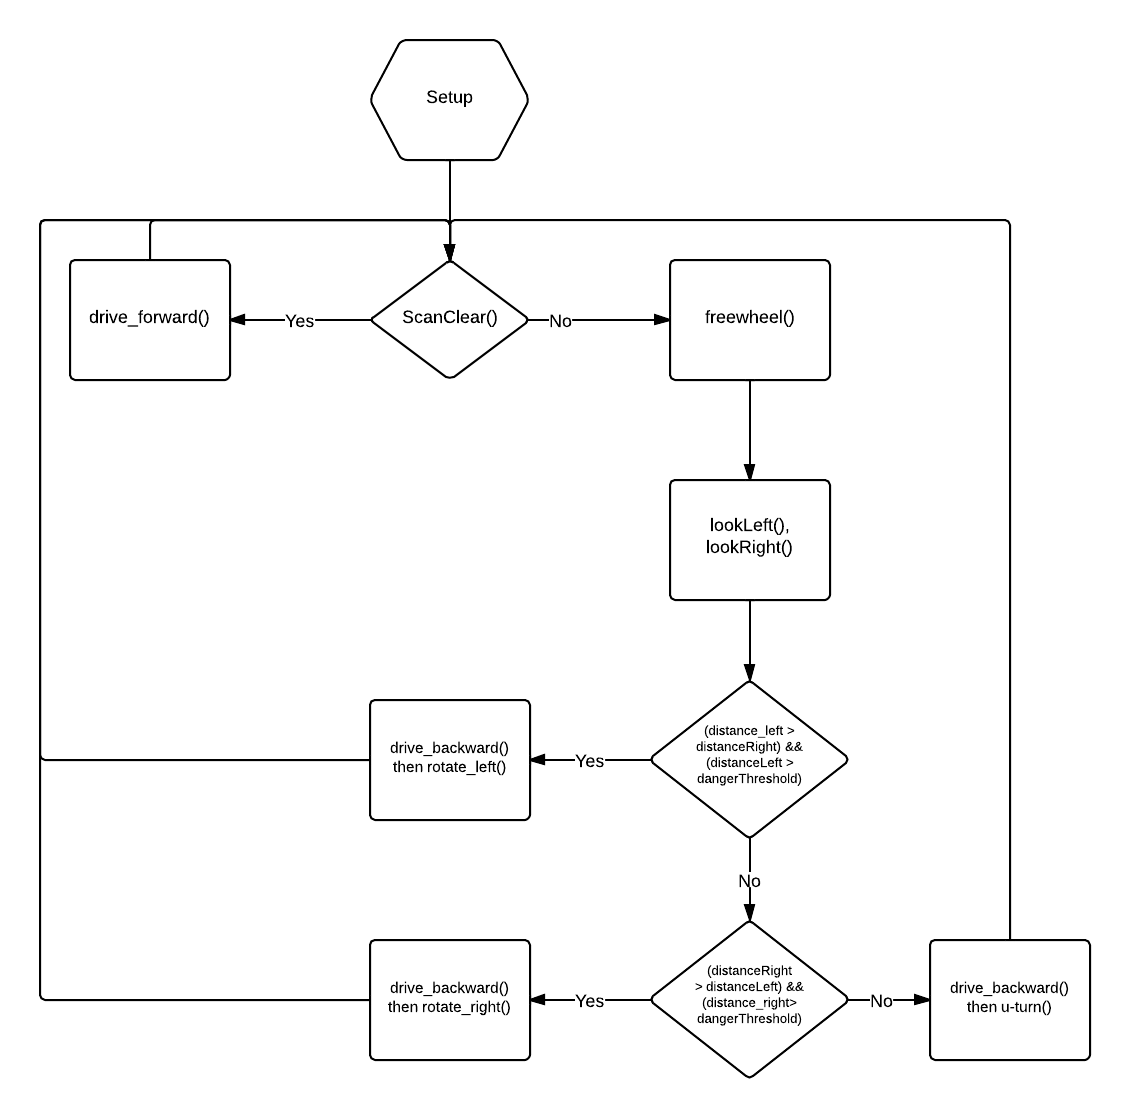
\includegraphics[height=0.85\textwidth]{images/main.png}
	\caption{Main Loop Flowchart}
		\label{main}
	\end{figure}


	\begin{figure}[b]\centering
	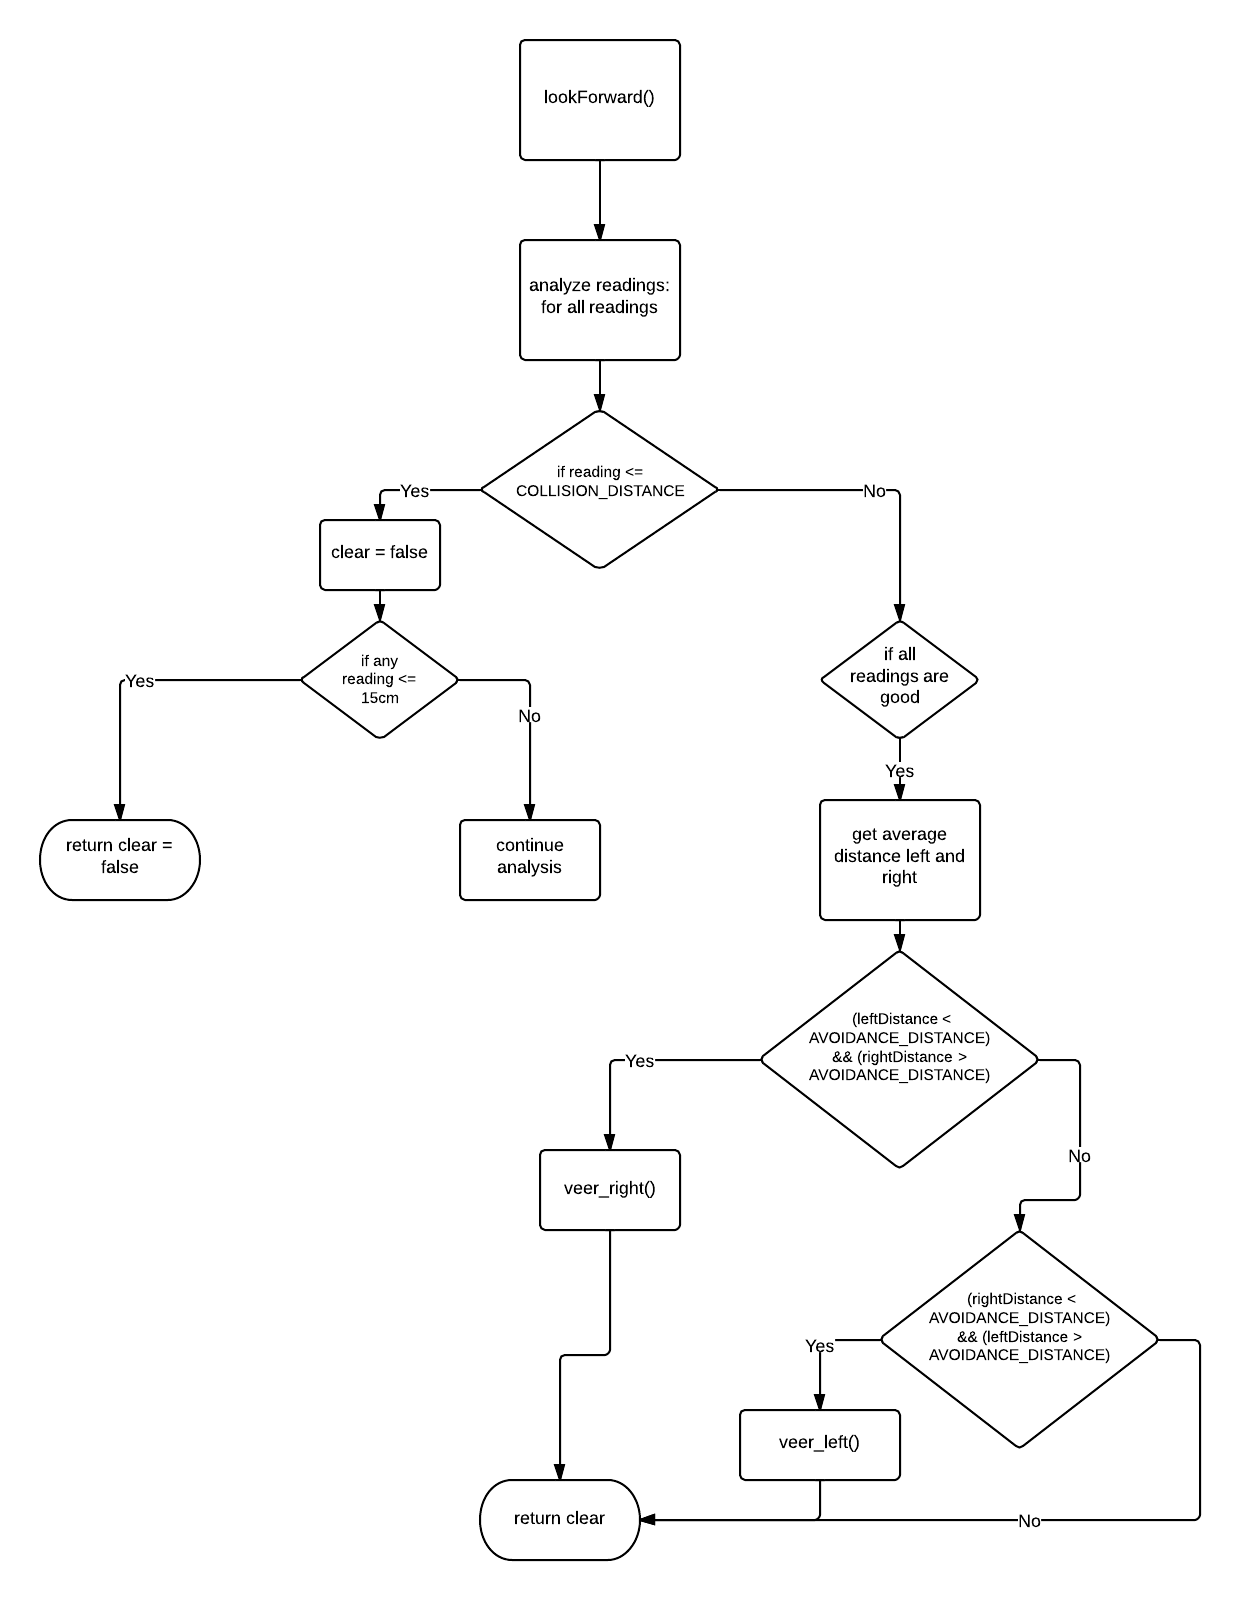
\includegraphics[height=0.85\textwidth]{images/scan_clear.png}
	\caption{scanClear() Flowchart}
		\label{scan}
	\end{figure}
	
\par\noindent
%TODO Caren or me: change main diagram (distanceRight instead of distance_right)

\newpage

 \begin{lstlisting}[caption=Control Loop, label=loop]		
  void loop() {
    if (scanClear())  drive_forward(); 
    else              // if path is blocked
    {
      freewheel();    // stop
      lookLeft();
      int distanceLeft = getAverageDistance();

      lookRight();
      int distanceRight = getAverageDistance();
      
      servo_position(CENTER);

      // go the least obstructed way
      if (distanceLeft > distanceRight && distanceLeft > dangerThreshold)       
      {
        drive_backward();
        delay(400);
        rotate_left();
      }
      else if (distanceRight > distanceLeft && distanceRight > dangerThreshold) 
      {
        drive_backward();
        delay(400);
        rotate_right();
      }
      else 		// equally blocked or less than danger threshold left or right
      {
        freewheel();
        delay(20);
        drive_backward();
        delay(500);
        u_turn();
      }   
    } 
  }  
  }
  \end{lstlisting}



The primary purpose of our program is to ensure that SaMMY avoids all obstacles. Figure \ref{main} shows how our code is structured, and Listing \ref{loop} provides a code snippet from the main loop.
Once the setup has run and the components have been initialized, the program enters the main section of our program and runs in an infinite loop which scans for objects and makes decisions on which direction to go. First, the \texttt{scanClear()} function is called, which checks for objects in front of the robot within a 40\degree \hspace{1pt} angle width. If this value is \emph{True}, the area is clear and the robot drives forward. Otherwise, it stops, calls \texttt{lookLeft()} and \texttt{lookRight()} and calculates the average distance to each side. If \texttt{distanceLeft} is greater than \texttt{distanceRight} and greater than \texttt{dangerThreshold}, the bot backs up and rotates left. Likewise, if \texttt{distanceRight} is greater than \texttt{distanceLeft} and greater than the \texttt{dangerThreshold}, the bot backs up and rotates right. Otherwise, it is blocked on both sides. At this point it backs up and makes a U-turn.


To add some character to our robot, we added a counter that would launch SaMMY into a ``victory dance''.  We check this value before launching the \texttt{scanClear()} function.  If it's time to dance, then the \texttt{coolness()} function is called and SaMMY performs his victory dance.
%\par\noindent

Figure \ref{scan} shows a more detailed flowchart of the algorithm for \texttt{scanClear()}, which is called at the start of every loop.
  
%TODO Caren collision distance confusing - doesn't go anywhere in diagram when continue analysis happens.  
% Why do we not return immediately when collision distance detected?



This function calls \texttt{lookForward()}, which returns 5 readings at 10\degree \hspace{1pt} increments. If any of these distances is less than \texttt{COLLISION\_DISTANCE}, the \texttt{clear} flag is set to \emph{FALSE} and \texttt{EMERGENCY\_DISTANCE} is checked. If the value is below the emergency distance, the program immediately returns \emph{FALSE} so that the appropriate action can be taken. Otherwise, the program function finishes its analysis and then returns the \texttt{clear} value.
Provided the \texttt{clear} flag is \emph{TRUE}, the robot then checks for the average distance on the left and right. If exactly one side's distance is less than \texttt{AVOIDANCE\_DISTANCE} (the first and therefore farthest distance the bot checks) it veers the opposite way and continues driving forward. Once \texttt{scanClear()} has finished, it returns the \texttt{clear} value and the next actions are taken (Figure \ref{main}).

%The look functions set up the angles and call the scan() function.
%TODO Caren talk about look functions or ignore?
The \texttt{scan()} function actually performs the scans at each angle by sending a sonar ``ping'' and waiting for the return signal to measure the distance. Sometimes the sonar returns very low, erroneous values that would cause the robot to halt. To avoid that, the \texttt{scan()} function only stops the bot and re-centers the sonar if two ping results in a row are below the emergency distance. 

%TODO create "performance" or "results" section, or just lump it in with conclusion?




  

\section{Conclusion}
\texttt{Servo and Protecto} was quite fun for us to build and was certainly the biggest ``crowd pleaser'' out of all the projects we've made.  The assembly perhaps took the least amount of time, although we did face problems with a few of the parts not being built correctly (mainly the battery holder and motor plate mount).  Fixing the power problems was the most frustrating part of the project, but once we finished everything, the final product was quite rewarding.  We both spent equal times on all the different aspects of this project.  Currently, SaMMY performs quite well, even if he does run into walls occasionally.  This is caused by veering, which was a tough issue to fix. Listed below are some of the challenges we faced.
	
	\subsection{Challenges}
		
		\begin{itemize}				
		\item \textbf{Power Issues}: After the initial assembly, we were not able to properly move the servo and control the motors.  Our initial thought was inadequate power, but the correspondent we communicated with ensured us that it could run perfectly fine on 6V of AA batteries.  Even after upping the voltage we saw problems, which were due to the power demands of our servo.  After increasing the power to 9V of AA batteries the problem diminished.
		\item \textbf{Motor control}: The motors we received are not precise enough to deliver equal power on both sides.  This caused inevitable veering of the robot.  We were able to use our own veering function to correct a lot of this, but were not able to control the bot perfectly.
		\item \textbf{CMUcam}: We were able to calibrate and test the CMUcam, which was intended for color detection.  However, communicating the frames from the camera to the Arduino proved difficult.  Even the example code would not work on our device. We were not able to solve the communication error before the project was due.
		\item \textbf{Erroneous Sonar Readings}: Occasionally the ultrasonic sensor picked up incorrect values distance values that would immediately cause our bot to stop (possibly due to ghost echoes).  We adjusted this by waiting until it received two pings below 10cm.
		\end{itemize}

\subsection{Future Additions}
The Arduino platform and components in this project provide a large amount of functionality.  Because of this, the amount of improvements is virtually limitless.  Our goals in the future could involve adding:
		\begin{itemize}				
		\item \textbf{Battery Pack}: Buying a powerful, rechargeable battery pack would save money, improve performance and decrease hassle.
		\item \textbf{External Apparatus}: We initially wanted to attach a simple device that could be triggered based on certain events.  While launching or shooting an object would have been interesting, in most cases this would require PID algorithms, which would involve sufficiently more work and tuning.
		\item \textbf{Color Detection}: One of our original ideas (and part of the reason for the name \textbf{Servo and Protecto}) was to use color detection to differentiate between ``friends'' and ``enemies''.  There would be certain objects that the robot would purposely avoid, and others that it would just run over.
		\item \textbf{Infrared}: Infrared sensors can be used to detect edges, and they could also be used as an external controller/remote.
		\item \textbf{Object Following}: The sonar and/or color detector could be used to follow an object instead of avoid them.  This would be useful when if we attached a physical arm or apparatus of some sort.
		\end{itemize}


\section{References}
%TODO

	\begin {table}[h]
	\begin {center} 
	\vspace{15pt}
	
	\begin{tabular}{||c|c|l||}\hline	
		\textbf{Source}	&	\textbf{Description}	&	\textbf{Link}		\\\hline
		\multirow{3}{*}{Arduino Libraries}
						&	Servo		&	\url{http://bit.ly/1nuXP2Y} 		\\
						&	Sonar		&	\url{http://bit.ly/1pYs3OV} 		\\
						&	Motor		&	\url{http://bit.ly/1pepI2n}	 	\\\hline
		\multirow{2}{*}{Oddwires Robot Kit}
						&	Kit Description		&	 \url{http://bit.ly/TysmCv} \\
					&	Assembly Instructions		&	\url{http://bit.ly/1xASGf2} \\\hline

	\end{tabular}
		\caption {Robot Functions} \label{refs}
	\end{center}
	\end{table} 	

\end{document}
%references
%-oddwires
%-arduino
%Acknowledgement: this algorithm is based on the functions and sample sketch provided by oddWires with the purchase of the oddWires Arduino Kit.
%                 We used the idea behind the code but we repurposed the functions and used our own algorithms which basically made the bot behave 
%                 better in emergency situations and avoid obstacles in a smoother way. 
